\documentclass[conference]{IEEEtran}
\IEEEoverridecommandlockouts

% ---------- Packages ----------
\usepackage{cite}
\usepackage{amsmath,amssymb,amsfonts,amsthm}
\usepackage{algorithm}
\usepackage{algpseudocode}
\usepackage{graphicx}
\usepackage{textcomp}
\usepackage{xcolor}
\usepackage{booktabs}
\usepackage{array}
\usepackage{tikz}
\usetikzlibrary{arrows.meta,positioning,shapes.geometric,fit,calc}
\usepackage{pgfplots}
\pgfplotsset{compat=1.16}
\usepackage[hidelinks]{hyperref}

\def\BibTeX{{\rm B\kern-.05em{\sc i\kern-.025em b}\kern-.08em
    T\kern-.1667em\lower.7ex\hbox{E}\kern-.125em X}}

% ---------- Macros ----------
\newcommand{\E}{\mathbb{E}}
\newcommand{\pdata}{p_{\mathrm{data}}}
\newcommand{\pg}{p_{g}}
\newcommand{\pz}{p_{z}}
\newcommand{\thg}{\theta_g}
\newcommand{\thd}{\theta_d}
\newcommand{\JS}{\mathrm{JS}}
\newcommand{\KL}{\mathrm{KL}}
\newcommand{\norm}[1]{\left\lVert #1 \right\rVert}
\DeclareMathOperator*{\argmax}{arg\,max}
\DeclareMathOperator*{\argmin}{arg\,min}

\theoremstyle{plain}
\newtheorem{proposition}{Proposition}
\newtheorem{theorem}{Theorem}
\newtheorem{lemma}{Lemma}
\theoremstyle{definition}
\newtheorem{definition}{Definition}
\newtheorem{example}{Example}

\begin{document}

\title{Generative Adversarial Networks: Mathematical Foundations, Training Dynamics, Architectural Advances, and Applications}


\maketitle

% =====================================================
\begin{abstract}
Generative Adversarial Networks (GANs) learn to sample from a complex data distribution through a two-player game between a generator, which maps latent noise to synthetic samples, and a discriminator, which tries to distinguish synthetic samples from real ones. This report presents a self-contained study of GANs built around four influential papers: the original GAN formulation of Goodfellow et al.\ \cite{goodfellow2014gan}, the deep convolutional architecture guidelines of Radford et al.\ (DCGAN) \cite{radford2016dcgan}, the Wasserstein GAN of Arjovsky et al.\ \cite{arjovsky2017wgan}, and the style-based generator of Karras et al.\ (StyleGAN) \cite{karras2019stylegan}. We derive the adversarial objective from first principles, prove that the optimal discriminator leads to a Jensen--Shannon divergence criterion, interpret the global optimum as a Nash equilibrium, and analyse the alternating training algorithm together with its failure modes (vanishing gradients, mode collapse, and oscillatory dynamics). We then compare DCGAN, conditional GAN, WGAN, WGAN-GP and StyleGAN in terms of architecture, mathematical improvements, and empirical advantages, and survey applications in image synthesis, super-resolution, image-to-image translation, data augmentation, medical imaging, and synthetic tabular data. Diagrams, derivations, and comparison tables are provided throughout.
\end{abstract}

\begin{IEEEkeywords}
Generative adversarial networks, minimax optimization, Jensen--Shannon divergence, Wasserstein distance, DCGAN, StyleGAN, deep generative models.
\end{IEEEkeywords}

% =====================================================
\section{Introduction}
Generative modelling aims to learn a model distribution $\pg$ that approximates an unknown data distribution $\pdata$ given only a finite set of samples. Classical approaches such as Boltzmann machines, deep belief networks, and autoregressive models require explicit density models, Markov chain sampling, or intractable partition functions. Variational autoencoders (VAEs) \cite{kingma2014vae} optimise a lower bound on the likelihood but often produce blurry samples.

Goodfellow et al.\ \cite{goodfellow2014gan} proposed a different principle: \emph{implicit} generative modelling through a game. A generator $G$ transforms noise into samples, and a discriminator $D$ is trained to detect fakes; $G$ improves by fooling $D$. No density is ever written down, and neither Markov chains nor approximate inference are needed---only backpropagation.

\textbf{Scope and paper selection.} This report analyses four papers (Table~\ref{tab:papers}), selected because each marks a distinct stage of GAN research: (i) the foundational framework, (ii) the first widely adopted stable convolutional architecture, (iii) a principled change of divergence with a new theory of convergence, and (iv) a state-of-the-art generator design with controllable synthesis. Further works (cGAN \cite{mirza2014cgan}, WGAN-GP \cite{gulrajani2017wgangp}, and application papers) are discussed as supporting material.

\begin{table}[t]
\centering
\caption{The Four Core Papers Analysed}
\label{tab:papers}
\footnotesize
\begin{tabular}{@{}p{0.9cm}p{1.4cm}p{4.9cm}@{}}
\toprule
\textbf{Ref.} & \textbf{Year} & \textbf{Main contribution} \\
\midrule
\cite{goodfellow2014gan} & 2014 & Adversarial framework; minimax objective; JS-divergence analysis; training algorithm \\
\cite{radford2016dcgan} & 2015/16 & DCGAN: all-convolutional architecture and design rules enabling stable training; latent vector arithmetic \\
\cite{arjovsky2017wgan} & 2017 & WGAN: Earth-Mover distance, Kantorovich--Rubinstein dual, critic with Lipschitz constraint \\
\cite{karras2019stylegan} & 2019 & StyleGAN: mapping network, AdaIN style injection, noise inputs, style mixing \\
\bottomrule
\end{tabular}
\end{table}

The remainder of the report is organised as follows. Section~\ref{sec:fund} introduces fundamental concepts, Section~\ref{sec:math} derives the mathematical theory, Section~\ref{sec:train} studies training, Section~\ref{sec:arch} compares advanced architectures, Section~\ref{sec:app} surveys applications, and Section~\ref{sec:concl} concludes.

% =====================================================
\section{Fundamental Concepts}\label{sec:fund}

\subsection{Motivation}
Given i.i.d.\ samples $\{x_i\}_{i=1}^{N}\sim\pdata$ with $x\in\mathbb{R}^n$ (e.g., an image), maximum-likelihood training chooses a parametric density $p_\theta$ maximising $\sum_i\log p_\theta(x_i)$. For images, expressive densities are hard to normalise. GANs sidestep this: instead of evaluating $p_\theta(x)$, they define a \emph{sampler} $x=G(z)$ whose distribution $\pg$ is implicit. The learning signal comes from a trainable critic (the discriminator) rather than a fixed likelihood, so the notion of ``similar to data'' is itself learned, which helps produce sharp samples.

\subsection{Historical Development}
Table~\ref{tab:history} summarises key milestones. After the original GAN (2014), the main lines of progress were (a) architectural (DCGAN, progressive growing \cite{karras2018progan}, BigGAN \cite{brock2019biggan}, StyleGAN), (b) objective and regularisation (improved techniques \cite{salimans2016improved}, WGAN, WGAN-GP, spectral normalisation \cite{miyato2018spectral}), and (c) conditioning and translation (cGAN, pix2pix, CycleGAN). More recently diffusion models have surpassed GANs in sample quality on several benchmarks \cite{dhariwal2021diffusion}, though GANs remain attractive for single-pass, fast sampling.

\begin{table}[t]
\centering
\caption{Timeline of GAN Development}
\label{tab:history}
\footnotesize
\begin{tabular}{@{}p{0.9cm}p{6.3cm}@{}}
\toprule
\textbf{Year} & \textbf{Milestone} \\
\midrule
2014 & GAN \cite{goodfellow2014gan}; conditional GAN \cite{mirza2014cgan} \\
2015--16 & DCGAN \cite{radford2016dcgan}; improved training techniques \cite{salimans2016improved} \\
2017 & Principled training \cite{arjovsky2017principled}; WGAN \cite{arjovsky2017wgan}; WGAN-GP \cite{gulrajani2017wgangp}; SRGAN, pix2pix, CycleGAN \cite{ledig2017srgan,isola2017pix2pix,zhu2017cyclegan} \\
2018 & Progressive GAN \cite{karras2018progan}; spectral norm \cite{miyato2018spectral} \\
2019 & BigGAN \cite{brock2019biggan}; StyleGAN \cite{karras2019stylegan} \\
2020 & StyleGAN2 \cite{karras2020stylegan2} \\
\bottomrule
\end{tabular}
\end{table}

\subsection{Architecture and Roles of the Two Networks}
A GAN has two differentiable functions (typically deep neural networks), shown in Fig.~\ref{fig:gan}.

\textbf{Generator} $G(z;\thg)$: maps a latent vector $z\sim\pz$ (commonly $\mathcal{N}(0,I)$ or $\mathcal{U}[-1,1]$) to data space. Its output distribution is $\pg$, the push-forward of $\pz$ through $G$. The generator never sees real data directly; it learns only through gradients flowing back from $D$.

\textbf{Discriminator} $D(x;\thd)\in(0,1)$: a binary classifier estimating the probability that $x$ came from $\pdata$ rather than from $\pg$.

\textbf{Competition.} $D$ is rewarded for correct classification; $G$ is rewarded when $D$ errs on generated samples. The standard analogy: $G$ is a counterfeiter and $D$ is the police. As $D$ improves, $G$ must produce more realistic fakes; as $G$ improves, $D$ must discover finer cues. Ideally the process ends when fakes are indistinguishable from real data and $D$ outputs $1/2$ everywhere.

\begin{figure}[t]
\centering
\resizebox{\columnwidth}{!}{%
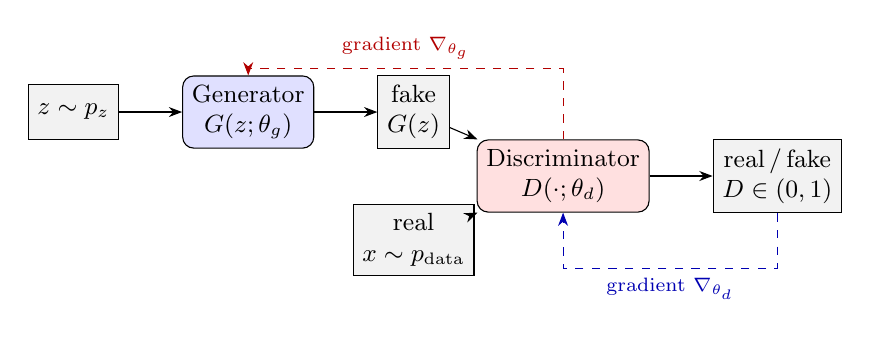
\begin{tikzpicture}[>=Stealth, node distance=7mm and 8mm,
  box/.style={draw, rounded corners, minimum height=8mm, minimum width=13mm, align=center, font=\small},
  io/.style={draw, minimum height=7mm, align=center, font=\small, fill=gray!10}]
  \node[io] (z) {$z\sim p_z$};
  \node[box, fill=blue!12, right=of z] (G) {Generator\\$G(z;\theta_g)$};
  \node[io, right=of G] (xf) {fake\\$G(z)$};
  \node[io, below=of xf] (xr) {real\\$x\sim p_{\mathrm{data}}$};
  \node[box, fill=red!12, right=of $(xf)!0.5!(xr)$] (D) {Discriminator\\$D(\cdot;\theta_d)$};
  \node[io, right=of D] (out) {real\,/\,fake\\$D\in(0,1)$};
  \draw[->] (z)--(G);
  \draw[->] (G)--(xf);
  \draw[->] (xf)--(D);
  \draw[->] (xr)--(D);
  \draw[->] (D)--(out);
  \draw[->, dashed, red!70!black] (D.north) -- ++(0,0.9) -| node[pos=0.25, above, font=\scriptsize]{gradient $\nabla_{\theta_g}$} (G.north);
  \draw[->, dashed, blue!70!black] (out.south) -- ++(0,-0.7) -| node[pos=0.25, below, font=\scriptsize]{gradient $\nabla_{\theta_d}$} (D.south);
\end{tikzpicture}}
\caption{GAN framework. $D$ receives real and generated samples and is trained to classify them; $G$ is updated by gradients propagated through $D$.}
\label{fig:gan}
\end{figure}

% =====================================================
\section{Mathematical Foundations}\label{sec:math}
We follow the notation of \cite{goodfellow2014gan}.

\subsection{Distributions, Noise, and Network Functions}
\begin{itemize}
\item $\pdata(x)$: the unknown true data density on $\mathcal{X}\subseteq\mathbb{R}^n$.
\item $\pz(z)$: a fixed, simple prior on $\mathcal{Z}\subseteq\mathbb{R}^d$; $z$ is the \emph{latent noise vector}.
\item $G:\mathcal{Z}\to\mathcal{X}$, $x=G(z;\thg)$. The induced density $\pg$ satisfies, for a differentiable invertible $G$, $\pg(x)=\pz(G^{-1}(x))\,|\det J_{G^{-1}}(x)|$; in general $G$ is not invertible and $\pg$ may be supported on a low-dimensional manifold, a fact that matters in Section~\ref{sec:train}.
\item $D:\mathcal{X}\to(0,1)$, $D(x;\thd)=\sigma(a(x;\thd))$, where $a$ is the pre-activation (logit) and $\sigma(u)=1/(1+e^{-u})$.
\end{itemize}

\subsection{Discriminator as a Probabilistic Classifier}
Label real samples $y=1$ and generated samples $y=0$, with equal priors. The discriminator models $D(x)=P(y=1\mid x)$. Its Bernoulli log-likelihood over a balanced dataset is
\begin{equation}
\E_{x\sim\pdata}[\log D(x)]+\E_{x\sim\pg}[\log(1-D(x))].
\label{eq:bce}
\end{equation}
Using the law of the unconscious statistician, $\E_{x\sim\pg}[f(x)]=\E_{z\sim\pz}[f(G(z))]$, this is exactly the value function
\begin{equation}
V(D,G)=\E_{x\sim\pdata}[\log D(x)]+\E_{z\sim\pz}[\log(1-D(G(z)))].
\label{eq:value}
\end{equation}

\subsection{Minimax Objective}
$D$ maximises $V$ (classification accuracy), while $G$ minimises it (making $D$ fail on fakes):
\begin{equation}
\min_{G}\max_{D}V(D,G).
\label{eq:minimax}
\end{equation}
This is a two-player zero-sum game with payoff $V$ for $D$ and $-V$ for $G$. Note the first term of $V$ does not depend on $G$.

\subsection{Optimal Discriminator}
\begin{proposition}[\cite{goodfellow2014gan}]\label{prop:Dstar}
For fixed $G$, the optimal discriminator is
\begin{equation}
D^*_G(x)=\frac{\pdata(x)}{\pdata(x)+\pg(x)}.
\label{eq:Dstar}
\end{equation}
\end{proposition}
\begin{proof}
Rewrite \eqref{eq:value} as an integral over $x$:
\begin{align}
V(D,G)&=\int_{x}\pdata(x)\log D(x)\,dx+\int_{z}\pz(z)\log(1-D(G(z)))\,dz \nonumber\\
&=\int_{x}\big[\pdata(x)\log D(x)+\pg(x)\log(1-D(x))\big]dx.
\end{align}
The integrand is, pointwise in $x$, a function $f(y)=a\log y+b\log(1-y)$ with $y=D(x)$, $a=\pdata(x)$, $b=\pg(x)$. For $(a,b)\neq(0,0)$, $f'(y)=a/y-b/(1-y)=0\Rightarrow y=a/(a+b)$, and $f''(y)=-a/y^2-b/(1-y)^2<0$, so this is the unique maximiser on $(0,1)$. Since $D$ may be chosen independently at each $x$ (assuming sufficient capacity), maximising the integrand at every $x$ maximises the integral. Outside $\mathrm{supp}(\pdata)\cup\mathrm{supp}(\pg)$ the value of $D$ does not affect $V$.
\end{proof}

\subsection{Reduction to the Jensen--Shannon Divergence}
Substitute \eqref{eq:Dstar} into the value function to obtain the \emph{virtual training criterion}
\begin{align}
C(G)&=\max_D V(D,G)=V(D^*_G,G)\nonumber\\
&=\E_{x\sim\pdata}\!\left[\log\frac{\pdata(x)}{\pdata(x)+\pg(x)}\right]\!+\!\E_{x\sim\pg}\!\left[\log\frac{\pg(x)}{\pdata(x)+\pg(x)}\right].
\label{eq:CG1}
\end{align}
Define the mixture $m(x)=\tfrac12(\pdata(x)+\pg(x))$. Then $\pdata/(\pdata+\pg)=\tfrac12\pdata/m$, so each logarithm contains a factor $\tfrac12$ contributing $\log\tfrac12=-\log2$ under each expectation:
\begin{align}
C(G)&=-\log 4+\KL(\pdata\,\|\,m)+\KL(\pg\,\|\,m)\nonumber\\
&=-\log4+2\,\JS(\pdata\,\|\,\pg),
\label{eq:CG2}
\end{align}
where $\KL(p\|q)=\int p\log(p/q)$ and $\JS(p\|q)=\tfrac12\KL(p\|m)+\tfrac12\KL(q\|m)$.

\begin{theorem}[Global optimum \cite{goodfellow2014gan}]
$C(G)$ attains its global minimum $-\log4$ if and only if $\pg=\pdata$.
\end{theorem}
\begin{proof}
$\JS(p\|q)\ge0$ with equality iff $p=q$ (it is a sum of non-negative KL terms, and $\KL(p\|m)=0$ iff $p=m$). Hence $C(G)\ge-\log4$ and equality holds iff $\pg=\pdata$. At that point $D^*_G(x)=1/2$ and $V=\log\tfrac12+\log\tfrac12=-\log4$.
\end{proof}

Thus, with an optimal discriminator, training the generator is equivalent to minimising the JS divergence, a symmetric, bounded ($0\le\JS\le\log2$) measure of distributional difference.

\subsection{Nash Equilibrium Interpretation}
A pair $(\thg^*,\thd^*)$ is a (pure) Nash equilibrium of the zero-sum game if neither player can improve by a unilateral deviation:
\begin{equation}
V(\thg^*,\thd)\le V(\thg^*,\thd^*)\le V(\thg,\thd^*)\quad\forall\,\thg,\thd,
\label{eq:saddle}
\end{equation}
i.e.\ $(\thg^*,\thd^*)$ is a saddle point of $V$. In the non-parametric setting, the pair $(\pg=\pdata,\;D\equiv\tfrac12)$ satisfies \eqref{eq:saddle}: (i) if $\pg=\pdata$ then every $D$ satisfies $V(D,G^*)=\E_{\pdata}[\log D]+\E_{\pdata}[\log(1-D)]\le-\log4$ by the concavity of $\log$ (the maximum is at $D=1/2$); (ii) with $D\equiv1/2$, $V(D^*,G)=-\log4$ for every $G$, so $G$ cannot improve on it. The value of the game is $-\log4\approx-1.386$.

\emph{Caveats.} The above holds in density space, where $V$ is convex in $\pg$ and concave in $D$. In parameter space, with neural networks, $V$ is generally non-convex in $\thg$ and non-concave in $\thd$, so equilibria need not exist or be reachable \cite{mescheder2018converge}. Gradient dynamics may cycle, as shown in Section~\ref{sec:train}.

\subsection{Practical Loss Functions}
With minibatches of size $m$, the discriminator minimises the binary cross-entropy
\begin{equation}
\mathcal{L}_D=-\frac1m\sum_{i=1}^{m}\Big[\log D(x^{(i)})+\log\big(1-D(G(z^{(i)}))\big)\Big].
\label{eq:LD}
\end{equation}
The \emph{saturating} generator loss from the minimax game is
\begin{equation}
\mathcal{L}_G^{\mathrm{sat}}=\frac1m\sum_{i=1}^{m}\log\big(1-D(G(z^{(i)}))\big),
\label{eq:LGsat}
\end{equation}
while \cite{goodfellow2014gan} recommends the \emph{non-saturating} loss
\begin{equation}
\mathcal{L}_G^{\mathrm{ns}}=-\frac1m\sum_{i=1}^{m}\log D(G(z^{(i)})).
\label{eq:LGns}
\end{equation}
Both share the same fixed point (they are both minimised when $D(G(z))\to1$) but provide different gradients; see Section~\ref{sec:train}-B.

\subsection{Wasserstein Distance (for WGAN)}
\begin{definition}
The Wasserstein-1 (Earth-Mover) distance between distributions $\mathbb{P}_r,\mathbb{P}_g$ is
\begin{equation}
W(\mathbb{P}_r,\mathbb{P}_g)=\inf_{\gamma\in\Pi(\mathbb{P}_r,\mathbb{P}_g)}\E_{(x,y)\sim\gamma}\big[\norm{x-y}\big],
\label{eq:w1}
\end{equation}
where $\Pi$ is the set of joint distributions (couplings) with marginals $\mathbb{P}_r$ and $\mathbb{P}_g$.
\end{definition}
Intuitively, $\gamma(x,y)$ is a plan describing how much probability mass is moved from $x$ to $y$, and $W$ is the cost of the cheapest plan. The infimum is intractable; the Kantorovich--Rubinstein duality \cite{villani2009optimal} gives
\begin{equation}
W(\mathbb{P}_r,\mathbb{P}_g)=\sup_{\norm{f}_L\le1}\ \E_{x\sim\mathbb{P}_r}[f(x)]-\E_{x\sim\mathbb{P}_g}[f(x)],
\label{eq:kr}
\end{equation}
where the supremum is over all $1$-Lipschitz functions, $|f(x)-f(y)|\le\norm{x-y}$. WGAN parameterises $f$ by a neural \emph{critic} $f_w$ and solves
\begin{equation}
\min_{\thg}\ \max_{w\in\mathcal{W}}\ \E_{x\sim\pdata}[f_w(x)]-\E_{z\sim\pz}[f_w(G(z))].
\label{eq:wgan}
\end{equation}
If the parameter set $\mathcal{W}$ is compact, all $f_w$ are $K$-Lipschitz for some $K$ and the maximum equals $K\cdot W$ up to a constant, which is sufficient for gradient purposes \cite{arjovsky2017wgan}. Under mild assumptions (generator continuous in $\thg$ and locally Lipschitz) the gradient exists almost everywhere and equals
\begin{equation}
\nabla_{\thg}W(\mathbb{P}_r,\mathbb{P}_{\thg})=-\E_{z\sim\pz}\big[\nabla_{\thg}f(G(z;\thg))\big],
\label{eq:wgrad}
\end{equation}
where $f$ is the optimal critic.

\subsection{Conditional GAN Objective}
For class labels or other side information $y$, the conditional GAN \cite{mirza2014cgan} feeds $y$ to both networks:
\begin{equation}
\min_G\max_D\ \E_{x\sim\pdata}[\log D(x|y)]+\E_{z\sim\pz}[\log(1-D(G(z|y)|y))].
\label{eq:cgan}
\end{equation}
The optimal discriminator becomes $D^*(x|y)=\pdata(x|y)/(\pdata(x|y)+\pg(x|y))$, and the same derivation shows that $G$ minimises the expected conditional JS divergence.

% =====================================================
\section{Training Mechanism}\label{sec:train}

\subsection{Alternating Optimisation Algorithm}
Because $\max_D$ cannot be solved exactly inside every generator step, \cite{goodfellow2014gan} alternates $k$ discriminator updates with one generator update (Algorithm~\ref{alg:gan}).

\begin{algorithm}[t]
\caption{Minibatch SGD training of GANs \cite{goodfellow2014gan}}
\label{alg:gan}
\begin{algorithmic}[1]
\For{each training iteration}
  \For{$k$ steps}
    \State Sample noise $\{z^{(i)}\}_{i=1}^m\sim\pz$ and data $\{x^{(i)}\}_{i=1}^m\sim\pdata$
    \State $\thd\leftarrow\thd+\eta\,\nabla_{\thd}\frac1m\sum_i\big[\log D(x^{(i)})+\log(1-D(G(z^{(i)})))\big]$
  \EndFor
  \State Sample noise $\{z^{(i)}\}_{i=1}^m\sim\pz$
  \State $\thg\leftarrow\thg-\eta\,\nabla_{\thg}\frac1m\sum_i\log(1-D(G(z^{(i)})))$ \Comment{or ascend $\log D(G(z))$}
\EndFor
\end{algorithmic}
\end{algorithm}

\subsection{Forward and Backward Propagation}
\textbf{Forward pass.} Real $x^{(i)}$ flows through $D$ to give $D(x^{(i)})=\sigma(a_r^{(i)})$; noise $z^{(i)}$ flows through $G$ to $\tilde x^{(i)}=G(z^{(i)})$, then through $D$ to give $D(\tilde x^{(i)})=\sigma(a_f^{(i)})$.

\textbf{Discriminator gradients.} Using $\sigma'(a)=\sigma(a)(1-\sigma(a))$, the derivatives of \eqref{eq:LD} with respect to the logits are
\begin{align}
\frac{\partial\mathcal{L}_D}{\partial a_r^{(i)}}&=-\frac1m\big(1-D(x^{(i)})\big),\\
\frac{\partial\mathcal{L}_D}{\partial a_f^{(i)}}&=\ \frac1m D(\tilde x^{(i)}),
\end{align}
which are then backpropagated through the layers of $D$ by the chain rule to give $\nabla_{\thd}\mathcal{L}_D$. The generator is held fixed.

\textbf{Generator gradients.} For the non-saturating loss \eqref{eq:LGns}, $\partial\mathcal{L}_G^{\mathrm{ns}}/\partial a_f^{(i)}=-\tfrac1m(1-D(\tilde x^{(i)}))$. The signal is backpropagated \emph{through $D$ to its input} and then into $G$:
\begin{equation}
\nabla_{\thg}\mathcal{L}_G=\sum_{i}\frac{\partial\mathcal{L}_G}{\partial a_f^{(i)}}\,\nabla_{x}a(\tilde x^{(i)};\thd)^{\!\top}\,\frac{\partial G(z^{(i)};\thg)}{\partial\thg},
\label{eq:chain}
\end{equation}
where $\partial G/\partial\thg$ is the Jacobian of the generator output. The discriminator weights are not updated in this step. This is why $D$ and $G$ must be differentiable and why the gradient of $D$ with respect to its \emph{input} is the quantity that teaches $G$.

\subsection{Vanishing Gradients}
For the saturating loss \eqref{eq:LGsat}, since $\partial\log(1-\sigma(a))/\partial a=-\sigma(a)=-D(\tilde x)$, the gradient at the logit is $-D(\tilde x)$. Early in training $G$ is poor, $D$ rejects fakes confidently, $D(\tilde x)\approx0$, and the gradient vanishes exactly when $G$ most needs it. The non-saturating loss instead has logit-gradient $-(1-D(\tilde x))\approx-1$ in that regime, restoring a strong signal.

A deeper cause is geometric \cite{arjovsky2017principled}. If $\pdata$ and $\pg$ are supported on low-dimensional manifolds (natural for images and for $G$ with $d\ll n$) that do not overlap, a perfect discriminator exists. Then $D^*$ is locally constant on each support, $\nabla_x D^*=0$ and the generator receives no useful gradient; moreover $\JS(\pdata\|\pg)=\log2$ is constant irrespective of how far apart the distributions are (Fig.~\ref{fig:jsw}). A too-good $D$ stalls $G$; a too-weak $D$ gives uninformative feedback.

\begin{figure}[t]
\centering
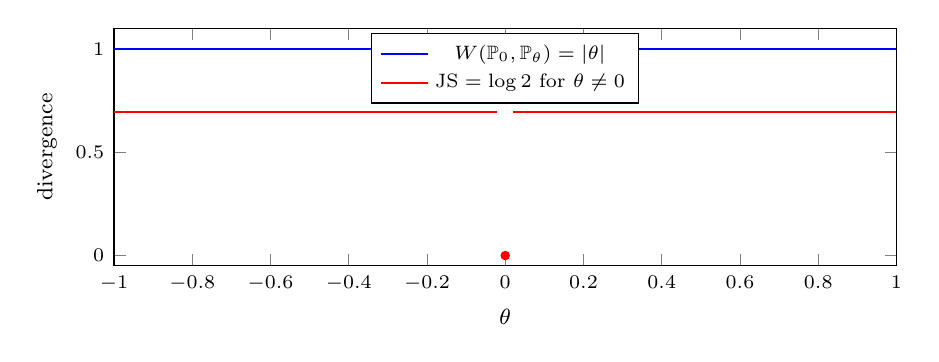
\begin{tikzpicture}
\begin{axis}[width=0.95\columnwidth,height=4.6cm,xlabel={$\theta$},ylabel={divergence},
  xmin=-1,xmax=1,ymin=-0.05,ymax=1.1,legend style={font=\scriptsize,at={(0.5,0.98)},anchor=north},
  tick label style={font=\scriptsize},label style={font=\footnotesize}]
\addplot[thick,blue,domain=-1:1,samples=2] {abs(x)};
\addlegendentry{$W(\mathbb{P}_0,\mathbb{P}_\theta)=|\theta|$}
\addplot[thick,red,domain=-1:-0.02,samples=2] {0.693};
\addplot[thick,red,domain=0.02:1,samples=2] {0.693};
\addlegendentry{$\mathrm{JS}=\log 2$ for $\theta\ne0$}
\addplot[only marks,mark=*,red,mark size=1.5pt] coordinates {(0,0)};
\end{axis}
\end{tikzpicture}
\caption{WGAN parallel-lines example \cite{arjovsky2017wgan}. $W$ is continuous and gives gradient everywhere; JS is discontinuous with zero gradient for $\theta\neq0$ (KL diverges).}
\label{fig:jsw}
\end{figure}

\begin{example}[Parallel lines \cite{arjovsky2017wgan}]
Let $Z\sim\mathcal{U}[0,1]$, $\mathbb{P}_0=(0,Z)$ and $\mathbb{P}_\theta=(\theta,Z)$ in $\mathbb{R}^2$. Then $W(\mathbb{P}_0,\mathbb{P}_\theta)=|\theta|$, $\JS=\log2$ and $\KL=+\infty$ for all $\theta\neq0$, and all are $0$ at $\theta=0$. Only $W$ is continuous in $\theta$ and provides a usable gradient.
\end{example}

\subsection{Mode Collapse}
Mode collapse occurs when $G$ maps many $z$ to a few outputs, covering only part of $\pdata$. One mechanism is the order of optimisation. The objective is $\min_G\max_D V$, but simultaneous gradient updates implicitly treat $\max_D\min_G V$. If the inner minimisation is solved first, $G$ moves all its mass to the point $x^*=\argmax_x D(x)$; $D$ then learns to reject $x^*$, $G$ jumps to the new maximum of $D$, and the cycle repeats without covering the distribution \cite{goodfellow2014gan,goodfellow2016tutorial}. Because the JS objective gives no direct penalty for missing modes (a loss of coverage can be compensated by sharp fakes), $G$ is not forced to diversify. Mitigations include minibatch discrimination and feature matching \cite{salimans2016improved}, the Wasserstein objective, gradient penalties, and conditioning.

\subsection{Instability and Convergence Challenges}
\textbf{Non-convergence of simultaneous gradient dynamics.} Consider the bilinear game $V(x,y)=xy$, in which $x$ (generator) minimises and $y$ (discriminator) maximises. Gradient descent--ascent with step $\eta$ gives
\begin{equation}
x_{t+1}=x_t-\eta y_t,\qquad y_{t+1}=y_t+\eta x_t,
\end{equation}
so $x_{t+1}^2+y_{t+1}^2=(1+\eta^2)(x_t^2+y_t^2)$: the iterates spiral \emph{outward} although $(0,0)$ is the unique equilibrium. In continuous time the trajectories are closed circles. Real GANs show analogous oscillation, because the Jacobian of the update field has eigenvalues with large imaginary parts \cite{mescheder2018converge}.

\textbf{Theory versus practice.} Proposition~2 of \cite{goodfellow2014gan} states that, if $G$ and $D$ have enough capacity, $D$ reaches its optimum for fixed $G$ at each step, and $\pg$ is updated to improve $C(G)=\max_D V(D,G)$, then $\pg\to\pdata$. The argument uses the fact that $V(D,G)=U(\pg,D)$ is convex in $\pg$, and the supremum of convex functions is convex, so descent on $\pg$ has a global optimum. In practice $G$ is updated in parameter space, not $\pg$ space, and the assumptions (optimal $D$, infinite capacity) are violated; this gap explains much of the instability.

\textbf{Other issues.} Sensitivity to hyper-parameters and initialisation, no meaningful loss curve (the discriminator loss is not a proxy for sample quality), and difficulty of evaluation. Common metrics are the Inception Score $\mathrm{IS}=\exp\big(\E_x\KL(p(y|x)\,\|\,p(y))\big)$ \cite{salimans2016improved} and the Fr\'echet Inception Distance
\begin{equation}
\mathrm{FID}=\norm{\mu_r-\mu_g}^2+\mathrm{Tr}\big(\Sigma_r+\Sigma_g-2(\Sigma_r\Sigma_g)^{1/2}\big),
\end{equation}
where $(\mu,\Sigma)$ are the mean and covariance of Inception features of real ($r$) and generated ($g$) samples \cite{heusel2017ttur}; lower FID is better.

% =====================================================
\section{Advanced GAN Architectures}\label{sec:arch}

\subsection{DCGAN \cite{radford2016dcgan}}
Original GANs used fully connected networks (with convolutions only in some experiments). Radford et al.\ identified architectural guidelines that made deep convolutional GANs train reliably:
\begin{itemize}
\item Replace pooling by \emph{strided convolutions} in $D$ and \emph{fractionally-strided (transposed) convolutions} in $G$, so the networks learn their own up/down-sampling.
\item Use \emph{batch normalisation} \cite{ioffe2015bn} in both networks (excluding $G$'s output layer and $D$'s input layer).
\item Remove fully connected hidden layers.
\item Use ReLU in $G$ (Tanh at the output) and LeakyReLU (slope $0.2$) in $D$.
\item Train with Adam \cite{kingma2015adam}, learning rate $2\times10^{-4}$ and $\beta_1=0.5$; weights from $\mathcal{N}(0,0.02^2)$.
\end{itemize}
A $100$-dimensional $z$ is projected and reshaped to a small spatial tensor, then up-sampled to $64\times64$ images (Fig.~\ref{fig:dcgan}). DCGAN does not change the objective \eqref{eq:minimax}; its contribution is architectural. It also showed that the latent space is structured: vector arithmetic on $z$ (e.g., ``smiling woman'' $-$ ``neutral woman'' $+$ ``neutral man'') yields semantically meaningful images, and discriminator features serve as unsupervised representations for classification.

\begin{figure}[t]
\centering
\resizebox{\columnwidth}{!}{%
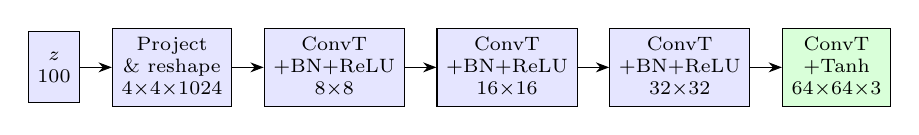
\begin{tikzpicture}[>=Stealth,node distance=4mm,
 b/.style={draw,minimum height=9mm,align=center,font=\scriptsize,fill=blue!10}]
 \node[b] (z) {$z$\\100};
 \node[b,right=of z] (p) {Project\\\& reshape\\$4{\times}4{\times}1024$};
 \node[b,right=of p] (c1) {ConvT\\+BN+ReLU\\$8{\times}8$};
 \node[b,right=of c1] (c2) {ConvT\\+BN+ReLU\\$16{\times}16$};
 \node[b,right=of c2] (c3) {ConvT\\+BN+ReLU\\$32{\times}32$};
 \node[b,right=of c3,fill=green!15] (o) {ConvT\\+Tanh\\$64{\times}64{\times}3$};
 \foreach \a/\b in {z/p,p/c1,c1/c2,c2/c3,c3/o} \draw[->](\a)--(\b);
\end{tikzpicture}}
\caption{DCGAN generator. The discriminator mirrors this with strided convolutions, BatchNorm, and LeakyReLU.}
\label{fig:dcgan}
\end{figure}

\subsection{Conditional GAN (cGAN) \cite{mirza2014cgan}}
cGAN adds a conditioning variable $y$ (label, text embedding, or image) to both networks, optimising \eqref{eq:cgan}. In practice $y$ is concatenated with $z$ in $G$ and with $x$ (or with an intermediate feature map) in $D$. This allows controlled generation (e.g., ``generate digit 7'') and is the basis for image-to-image translation \cite{isola2017pix2pix}. Mathematically the model learns $\pg(x|y)\to\pdata(x|y)$.

\subsection{Wasserstein GAN \cite{arjovsky2017wgan}}
WGAN replaces JS by $W_1$ and the discriminator by a \emph{critic} $f_w:\mathcal{X}\to\mathbb{R}$ without a sigmoid. The critic loss is $\mathcal{L}_{f}=\E_{z}[f_w(G(z))]-\E_x[f_w(x)]$ and the generator loss is $-\E_z[f_w(G(z))]$, obtained from \eqref{eq:wgan}. The Lipschitz constraint is enforced by clipping weights to $[-c,c]$ ($c=0.01$) after each update. The critic is trained for $n_{\text{critic}}=5$ steps per generator step using RMSProp (lr $5\times10^{-5}$), because the critic should be near-optimal for the gradient \eqref{eq:wgrad} to be meaningful. Advantages reported in \cite{arjovsky2017wgan}: (i) the critic loss correlates with sample quality, giving a usable convergence indicator; (ii) improved stability and reduced mode collapse, with training working even without batch norm or with MLP generators; (iii) meaningful gradients when supports are disjoint. The limitation is that weight clipping biases the critic toward simple functions and can cause vanishing or exploding gradients; the authors themselves call clipping ``a terrible way'' to enforce Lipschitz continuity.

\subsection{WGAN-GP \cite{gulrajani2017wgangp}}
Instead of clipping, the Lipschitz constraint is softly enforced by penalising the critic's gradient norm. Because a differentiable $1$-Lipschitz function has $\norm{\nabla f}\le1$, and the optimal critic satisfies $\norm{\nabla f^*(\hat x)}=1$ almost everywhere along straight lines between coupled real and generated points \cite{gulrajani2017wgangp}, the loss is
\begin{align}
L&=\underbrace{\E_{\tilde x\sim\pg}[D(\tilde x)]-\E_{x\sim\pdata}[D(x)]}_{\text{Wasserstein estimate}}\nonumber\\
&\quad+\lambda\,\E_{\hat x\sim\mathbb{P}_{\hat x}}\big[(\norm{\nabla_{\hat x}D(\hat x)}_2-1)^2\big],
\label{eq:wgangp}
\end{align}
with $\hat x=\epsilon x+(1-\epsilon)\tilde x$, $\epsilon\sim\mathcal{U}[0,1]$ and $\lambda=10$. Batch normalisation is avoided in the critic (it couples samples in a batch, conflicting with the per-sample penalty); layer normalisation is used instead. Adam with $\beta_1=0$, $\beta_2=0.9$ is used. WGAN-GP trained a broad set of architectures (including 101-layer ResNets) with little tuning.

\subsection{StyleGAN \cite{karras2019stylegan}}
StyleGAN redesigns only the \emph{generator} (the loss is the non-saturating GAN loss; the discriminator and progressive growing follow \cite{karras2018progan}). Instead of feeding $z$ only at the input, the design (Fig.~\ref{fig:style}) has:
\begin{enumerate}
\item A \emph{mapping network} $f:\mathcal{Z}\to\mathcal{W}$, an 8-layer MLP producing an intermediate latent $w=f(z)$. $\mathcal{W}$ need not follow a fixed prior, so it can become less entangled than $\mathcal{Z}$.
\item A \emph{synthesis network} that starts from a learned constant $4\times4\times512$ tensor and applies convolutions at resolutions up to $1024^2$ (18 layers in total).
\item \emph{Adaptive instance normalisation} (AdaIN) \cite{huang2017adain} in every layer: with learned affine map $A$ giving $y=(y_s,y_b)=A(w)$,
\begin{equation}
\mathrm{AdaIN}(x_i,y)=y_{s,i}\,\frac{x_i-\mu(x_i)}{\sigma(x_i)}+y_{b,i},
\label{eq:adain}
\end{equation}
where $x_i$ is the $i$-th feature map; $w$ thereby controls the \emph{style} (scale and bias) of each channel at each resolution.
\item \emph{Noise inputs}: per-pixel Gaussian noise, scaled by learned per-channel factors, is added to feature maps, modelling stochastic detail (hair, freckles) separately from global structure.
\item \emph{Style mixing regularisation}: two latents $w_1,w_2$ are used in different layers during training so that adjacent styles do not co-adapt.
\item The \emph{truncation trick}, $w'=\bar w+\psi(w-\bar w)$, trades variety for fidelity at sampling time.
\end{enumerate}
Coarse resolutions ($4^2$--$8^2$) control pose and face shape, middle resolutions control facial features, and fine resolutions control colour and micro-structure. The paper also introduced the FFHQ dataset (70,000 images at $1024^2$) and the perceptual path length and linear separability metrics for disentanglement. On FFHQ, the FID improved from 8.04 for the progressive-GAN baseline to 4.40 for the full StyleGAN configuration \cite{karras2019stylegan}.

\begin{figure}[t]
\centering
\resizebox{\columnwidth}{!}{%
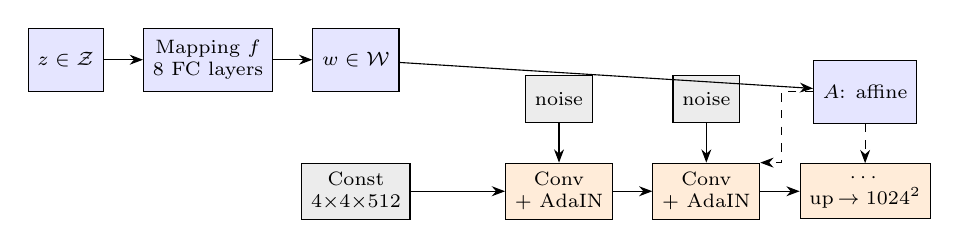
\begin{tikzpicture}[>=Stealth,node distance=5mm,
 b/.style={draw,minimum height=8mm,align=center,font=\scriptsize,fill=blue!10},
 s/.style={draw,minimum height=7mm,align=center,font=\scriptsize,fill=orange!15},
 n/.style={draw,minimum height=6mm,align=center,font=\scriptsize,fill=gray!15}]
 \node[b] (z) {$z\in\mathcal{Z}$};
 \node[b,right=of z] (m) {Mapping $f$\\8 FC layers};
 \node[b,right=of m] (w) {$w\in\mathcal{W}$};
 \node[n,below=9mm of w] (c) {Const\\$4{\times}4{\times}512$};
 \node[s,right=12mm of c] (s1) {Conv\\+ AdaIN};
 \node[s,right=of s1] (s2) {Conv\\+ AdaIN};
 \node[s,right=of s2] (s3) {$\cdots$\\up\,$\to1024^2$};
 \node[n,above=5mm of s1] (n1) {noise};
 \node[n,above=5mm of s2] (n2) {noise};
 \node[b,above=5mm of s3] (A) {$A$: affine};
 \draw[->](z)--(m);\draw[->](m)--(w);
 \draw[->](w)--(A);
 \draw[->](c)--(s1);\draw[->](s1)--(s2);\draw[->](s2)--(s3);
 \draw[->](n1)--(s1);\draw[->](n2)--(s2);
 \draw[->,dashed](A.south)--(s3.north);
 \draw[->,dashed](A.west)--++(-0.4,0)|-(s2.north east) ;
\end{tikzpicture}}
\caption{Simplified StyleGAN generator. The style vector $w$ is transformed by learned affine maps $A$ into AdaIN parameters at every layer; noise is injected separately.}
\label{fig:style}
\end{figure}

\subsection{Architecture Comparison}
\begin{table*}[t]
\centering
\caption{Comparison of Major GAN Variants}
\label{tab:compare}
\footnotesize
\renewcommand{\arraystretch}{1.15}
\begin{tabular}{@{}p{1.6cm}p{3.3cm}p{3.3cm}p{3.6cm}p{3.6cm}@{}}
\toprule
\textbf{Model} & \textbf{Architecture} & \textbf{Objective / divergence} & \textbf{Stabilisation} & \textbf{Advantages / limitations} \\
\midrule
GAN \cite{goodfellow2014gan} & MLP (some conv) $G$, $D$ & Minimax BCE; $\JS$ at optimal $D$ & Alternating $k{:}1$ updates; non-saturating loss & Simple, implicit model; unstable, mode collapse \\
cGAN \cite{mirza2014cgan} & $y$ fed to $G$ and $D$ & Conditional BCE \eqref{eq:cgan} & As GAN & Controllable generation; needs labels \\
DCGAN \cite{radford2016dcgan} & Strided/transposed conv, BN, ReLU/LReLU, no FC & Same as GAN & Architectural rules, Adam ($\beta_1{=}0.5$) & Stable $64^2$ images, latent arithmetic; objective unchanged \\
WGAN \cite{arjovsky2017wgan} & Critic w/o sigmoid & $W_1$ via KR dual \eqref{eq:wgan} & Weight clipping, $n_{\text{critic}}{=}5$, RMSProp & Meaningful loss, fewer collapses; clipping artefacts, slow \\
WGAN-GP \cite{gulrajani2017wgangp} & Critic w/o BN (LayerNorm) & $W_1$ + gradient penalty \eqref{eq:wgangp} & $\lambda{=}10$, Adam ($\beta_1{=}0$) & Robust across architectures; extra gradient cost \\
StyleGAN \cite{karras2019stylegan} & Mapping net, const input, AdaIN, noise, progressive growing & Non-saturating GAN loss (+ R1 in later versions) & Style mixing, truncation & State-of-the-art $1024^2$ faces, disentangled control; artefacts fixed in \cite{karras2020stylegan2} \\
\bottomrule
\end{tabular}
\end{table*}

Table~\ref{tab:compare} summarises these models. The progression shows two complementary strategies: \emph{changing what is optimised} (WGAN, WGAN-GP: from JS to $W_1$) and \emph{changing how the generator is built} (DCGAN, StyleGAN). State-of-the-art systems typically combine them, e.g., a convolutional generator, a regularised discriminator (gradient penalties or spectral normalisation \cite{miyato2018spectral}) and a non-saturating or Wasserstein-like loss.

% =====================================================
\section{Practical Applications}\label{sec:app}

\textbf{Image generation.} Large conditional models (BigGAN \cite{brock2019biggan}) generate high-fidelity class-conditional ImageNet images, and StyleGAN produces photorealistic faces and supports semantic editing by manipulating $w$ and style mixing.

\textbf{Super-resolution.} SRGAN \cite{ledig2017srgan} trains a generator to upscale low-resolution images by $4\times$, combining a perceptual (VGG feature) loss with an adversarial loss $\mathcal{L}=\mathcal{L}_{\text{content}}+10^{-3}\mathcal{L}_{\text{adv}}$. Pixel-wise MSE favours blurry averages; the adversarial term pushes outputs towards the natural-image manifold, yielding sharper textures at the cost of lower PSNR.

\textbf{Image-to-image translation.} Pix2pix \cite{isola2017pix2pix} is a conditional GAN for paired data (labels$\to$photo, edges$\to$photo) with objective $\mathcal{L}_{cGAN}+\lambda\mathcal{L}_{L1}$ and a patch-based discriminator. CycleGAN \cite{zhu2017cyclegan} handles unpaired domains using two generators and a cycle-consistency loss $\E_x\norm{F(G(x))-x}_1+\E_y\norm{G(F(y))-y}_1$.

\textbf{Data augmentation.} Generated samples enlarge small or imbalanced datasets and can improve classifier accuracy, e.g., DAGAN for few-shot learning \cite{antoniou2017dagan}. Gains depend on the diversity and fidelity of the samples; poorly trained GANs can inject artefacts.

\textbf{Medical imaging.} GANs are used for synthesis, cross-modality translation (MRI$\leftrightarrow$CT), denoising, and segmentation; see the review in \cite{yi2019medical}. Frid-Adar et al.\ \cite{fridadar2018liver} used classical augmentation followed by GAN-generated lesion patches to improve CNN liver-lesion classification (sensitivity and specificity increased relative to classical augmentation alone). Because synthetic data can mitigate scarcity and privacy constraints, it is attractive; however, validation by clinicians is needed to avoid hallucinated pathology.

\textbf{Synthetic data generation.} Beyond images, GANs create synthetic tabular records (CTGAN \cite{xu2019ctgan}, with mode-specific normalisation and conditional sampling for imbalanced categorical columns) and time series. Applications include privacy-preserving data sharing and testing.

\begin{table}[t]
\centering
\caption{Applications and Representative GAN Models}
\label{tab:apps}
\footnotesize
\renewcommand{\arraystretch}{1.1}
\begin{tabular}{@{}p{1.8cm}p{2.0cm}p{3.3cm}@{}}
\toprule
\textbf{Application} & \textbf{Model} & \textbf{Key mechanism} \\
\midrule
Image synthesis & DCGAN, BigGAN, StyleGAN & Conv./style-based generators \\
Super-resolution & SRGAN \cite{ledig2017srgan} & Perceptual + adversarial loss \\
Translation & pix2pix, CycleGAN & Conditional $D$; cycle loss \\
Augmentation & DAGAN \cite{antoniou2017dagan} & Conditional sample generation \\
Medical imaging & GAN-augmentation \cite{fridadar2018liver} & Lesion synthesis; modality translation \\
Tabular data & CTGAN \cite{xu2019ctgan} & Conditional vector; mode normalisation \\
\bottomrule
\end{tabular}
\end{table}

\textbf{Limitations and ethics.} The same technology enables deepfakes and biased synthetic data that reproduces dataset biases; evaluation with FID/IS does not guarantee downstream utility, and synthetic medical or personal data may leak information about training samples.

% =====================================================
\section{Conclusion}\label{sec:concl}
This report examined GANs through four landmark papers. The original GAN \cite{goodfellow2014gan} formulated generative modelling as a minimax game and showed that, with an optimal discriminator, the generator minimises $2\,\JS(\pdata\|\pg)-\log4$, with a Nash equilibrium at $\pg=\pdata$ and $D\equiv1/2$. Practical training, however, departs from the theory and suffers from vanishing gradients, mode collapse, and oscillatory dynamics. DCGAN \cite{radford2016dcgan} provided architectural design rules enabling stable convolutional training; WGAN \cite{arjovsky2017wgan}, and its gradient-penalty extension \cite{gulrajani2017wgangp}, replaced JS by the Wasserstein distance, giving continuous, informative gradients and a meaningful loss; StyleGAN \cite{karras2019stylegan} introduced a style-based generator that improves quality, stochastic detail, and controllability. Applications span image synthesis, super-resolution, translation, augmentation, medical imaging, and synthetic data.

Open challenges include rigorous convergence guarantees in non-convex games, reliable evaluation metrics, training with limited data, and responsible use. Future work may combine adversarial training with other generative families (e.g., diffusion models) to retain the fast sampling of GANs while improving mode coverage.

% =====================================================
\begin{thebibliography}{99}

\bibitem{goodfellow2014gan} I.~Goodfellow, J.~Pouget-Abadie, M.~Mirza, B.~Xu, D.~Warde-Farley, S.~Ozair, A.~Courville, and Y.~Bengio, ``Generative adversarial nets,'' in \emph{Proc. Adv. Neural Inf. Process. Syst. (NIPS)}, 2014, pp. 2672--2680.

\bibitem{radford2016dcgan} A.~Radford, L.~Metz, and S.~Chintala, ``Unsupervised representation learning with deep convolutional generative adversarial networks,'' in \emph{Proc. Int. Conf. Learn. Represent. (ICLR)}, 2016, arXiv:1511.06434.

\bibitem{arjovsky2017wgan} M.~Arjovsky, S.~Chintala, and L.~Bottou, ``Wasserstein generative adversarial networks,'' in \emph{Proc. Int. Conf. Mach. Learn. (ICML)}, 2017, pp. 214--223.

\bibitem{karras2019stylegan} T.~Karras, S.~Laine, and T.~Aila, ``A style-based generator architecture for generative adversarial networks,'' in \emph{Proc. IEEE/CVF Conf. Comput. Vis. Pattern Recognit. (CVPR)}, 2019, pp. 4401--4410.

\bibitem{mirza2014cgan} M.~Mirza and S.~Osindero, ``Conditional generative adversarial nets,'' arXiv:1411.1784, 2014.

\bibitem{gulrajani2017wgangp} I.~Gulrajani, F.~Ahmed, M.~Arjovsky, V.~Dumoulin, and A.~Courville, ``Improved training of Wasserstein GANs,'' in \emph{Proc. Adv. Neural Inf. Process. Syst. (NIPS)}, 2017, pp. 5767--5777.

\bibitem{arjovsky2017principled} M.~Arjovsky and L.~Bottou, ``Towards principled methods for training generative adversarial networks,'' in \emph{Proc. Int. Conf. Learn. Represent. (ICLR)}, 2017.

\bibitem{salimans2016improved} T.~Salimans, I.~Goodfellow, W.~Zaremba, V.~Cheung, A.~Radford, and X.~Chen, ``Improved techniques for training GANs,'' in \emph{Proc. Adv. Neural Inf. Process. Syst. (NIPS)}, 2016, pp. 2234--2242.

\bibitem{heusel2017ttur} M.~Heusel, H.~Ramsauer, T.~Unterthiner, B.~Nessler, and S.~Hochreiter, ``GANs trained by a two time-scale update rule converge to a local Nash equilibrium,'' in \emph{Proc. Adv. Neural Inf. Process. Syst. (NIPS)}, 2017, pp. 6626--6637.

\bibitem{mescheder2018converge} L.~Mescheder, A.~Geiger, and S.~Nowozin, ``Which training methods for GANs do actually converge?'' in \emph{Proc. Int. Conf. Mach. Learn. (ICML)}, 2018, pp. 3481--3490.

\bibitem{goodfellow2016tutorial} I.~Goodfellow, ``NIPS 2016 tutorial: Generative adversarial networks,'' arXiv:1701.00160, 2016.

\bibitem{karras2018progan} T.~Karras, T.~Aila, S.~Laine, and J.~Lehtinen, ``Progressive growing of GANs for improved quality, stability, and variation,'' in \emph{Proc. Int. Conf. Learn. Represent. (ICLR)}, 2018.

\bibitem{karras2020stylegan2} T.~Karras, S.~Laine, M.~Aittala, J.~Hellsten, J.~Lehtinen, and T.~Aila, ``Analyzing and improving the image quality of StyleGAN,'' in \emph{Proc. IEEE/CVF Conf. Comput. Vis. Pattern Recognit. (CVPR)}, 2020, pp. 8110--8119.

\bibitem{brock2019biggan} A.~Brock, J.~Donahue, and K.~Simonyan, ``Large scale GAN training for high fidelity natural image synthesis,'' in \emph{Proc. Int. Conf. Learn. Represent. (ICLR)}, 2019.

\bibitem{miyato2018spectral} T.~Miyato, T.~Kataoka, M.~Koyama, and Y.~Yoshida, ``Spectral normalization for generative adversarial networks,'' in \emph{Proc. Int. Conf. Learn. Represent. (ICLR)}, 2018.

\bibitem{ledig2017srgan} C.~Ledig \emph{et al.}, ``Photo-realistic single image super-resolution using a generative adversarial network,'' in \emph{Proc. IEEE Conf. Comput. Vis. Pattern Recognit. (CVPR)}, 2017, pp. 4681--4690.

\bibitem{isola2017pix2pix} P.~Isola, J.-Y.~Zhu, T.~Zhou, and A.~A.~Efros, ``Image-to-image translation with conditional adversarial networks,'' in \emph{Proc. IEEE Conf. Comput. Vis. Pattern Recognit. (CVPR)}, 2017, pp. 1125--1134.

\bibitem{zhu2017cyclegan} J.-Y.~Zhu, T.~Park, P.~Isola, and A.~A.~Efros, ``Unpaired image-to-image translation using cycle-consistent adversarial networks,'' in \emph{Proc. IEEE Int. Conf. Comput. Vis. (ICCV)}, 2017, pp. 2223--2232.

\bibitem{antoniou2017dagan} A.~Antoniou, A.~Storkey, and H.~Edwards, ``Data augmentation generative adversarial networks,'' arXiv:1711.04340, 2017.

\bibitem{fridadar2018liver} M.~Frid-Adar, I.~Diamant, E.~Klang, M.~Amitai, J.~Goldberger, and H.~Greenspan, ``GAN-based synthetic medical image augmentation for increased CNN performance in liver lesion classification,'' \emph{Neurocomputing}, vol.~321, pp. 321--331, 2018.

\bibitem{yi2019medical} X.~Yi, E.~Walia, and P.~Babyn, ``Generative adversarial network in medical imaging: A review,'' \emph{Med. Image Anal.}, vol.~58, art.~101552, 2019.

\bibitem{xu2019ctgan} L.~Xu, M.~Skoularidou, A.~Cuesta-Infante, and K.~Veeramachaneni, ``Modeling tabular data using conditional GAN,'' in \emph{Proc. Adv. Neural Inf. Process. Syst. (NeurIPS)}, 2019.

\bibitem{kingma2014vae} D.~P.~Kingma and M.~Welling, ``Auto-encoding variational Bayes,'' in \emph{Proc. Int. Conf. Learn. Represent. (ICLR)}, 2014.

\bibitem{kingma2015adam} D.~P.~Kingma and J.~Ba, ``Adam: A method for stochastic optimization,'' in \emph{Proc. Int. Conf. Learn. Represent. (ICLR)}, 2015.

\bibitem{ioffe2015bn} S.~Ioffe and C.~Szegedy, ``Batch normalization: Accelerating deep network training by reducing internal covariate shift,'' in \emph{Proc. Int. Conf. Mach. Learn. (ICML)}, 2015, pp. 448--456.

\bibitem{huang2017adain} X.~Huang and S.~Belongie, ``Arbitrary style transfer in real-time with adaptive instance normalization,'' in \emph{Proc. IEEE Int. Conf. Comput. Vis. (ICCV)}, 2017, pp. 1501--1510.

\bibitem{villani2009optimal} C.~Villani, \emph{Optimal Transport: Old and New}. Berlin, Germany: Springer, 2009.

\bibitem{dhariwal2021diffusion} P.~Dhariwal and A.~Nichol, ``Diffusion models beat GANs on image synthesis,'' in \emph{Proc. Adv. Neural Inf. Process. Syst. (NeurIPS)}, 2021.

\end{thebibliography}

\end{document}